  \chapter{\Kieker\ Monitoring Component}
    \section{Configuration}
      The monitoring part of \Kieker\ can be configured using the configuration file named ''\monitoringPropertiesFile``. This file should be copied for use to the directory ''META-INF`` of the own project and should - like the ''aop.xml`` - be copied during compiling. In order to inform \Kieker\ about this file, the following parameter should be used for the JVM:
      \begin{lstlisting}
	-Dkieker.monitoring.properties=META-INF/kieker.monitoring.properties
      \end{lstlisting}
      Most of the variables are self-explanatory and some of them will be explained in the following.

    \section{Monitoring Records}
      % They are not really only part of the monitoring components, but they have to be mentioned somehow.
      As we already saw, the records are the objects which store the monitored informations somehow. They are not really part of \KiekerMonitoring\ but in order to the use in the following, we will examine them.\\
      If we want to implement an own record, it should be extend the already existing class \textit{kieker.common.record.AbstractMonitoringRecord}. The record should be able to put his complete content into an array (of Object] so that the other components of \Kieker\ are able to persist and load the data and should of course provide a method to restore the content from an array. The following listing shows a simple record implementation which has fields for the class and the method that is called.
      \setJavaCodeListing
      \lstset{caption=MyRecord.java}
      \lstinputlisting{source-example/monitoring-and-analysis-with-own-components/src/mySimpleKiekerExample/bookstoreTracing/MyRecord.java}

    \section{Monitoring Probes}
      The probes are responsible for the decision which (and where) informations should be recorded. Technically we already implemented them by surrounding the method calls with the correct statements to clock, to produce the records and to deliver these records to the monitoring controller. Other specific controller could for example record only the amount of delivered bytes between methods or record only every second method call as well.\\
      We already used the annotations to make the monitoring much more comfortable and could also implement own annotations for AspectJ, but this won't be explained in this tutorial, because it would simply go beyond the scope.

    \section{Monitoring Log Writers}
      \hypertarget{monitoringlogwriters} 
      The so called \textit{monitoring log writers} (they can be seen as well in figure \ref{image:kiekercomponentdiagram}) are the parts of \Kieker\ which are responsible for writing and serializing the recorded informations into files, databases and so on. In other words: They get an instance of \textit{AbstractKiekerMonitoringRecord} and produce an output of any nature whatsoever.\\
      Of course there are already some writers implemented, as can be seen in figure \ref{image:writers}.
      % This is the diagram with the different types of writers.
      \begin{figure}[H]
	\begin{center}
	  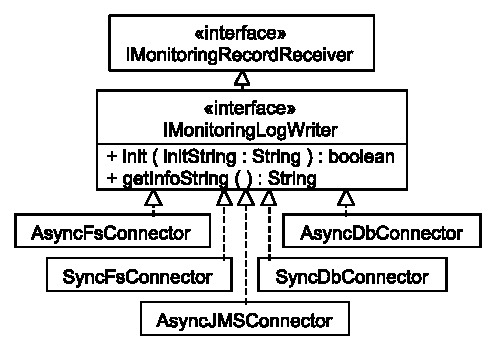
\includegraphics[width=0.5\textwidth]{./images/kieker_writerimpls.pdf}
	  \caption{The inheritance hierarchy of the current implemented monitoring log writers}
	  \label{image:writers}
	\end{center}
      \end{figure}
      As the quick start part already showed it, every monitored record is sent to the \textit{TpmonController} which itself calls the current writer. The writer uses for example the \textit{toArray()} method of the record to get the informations stored by the record as handable array. The writer is then able to write these objects for example into a file.\\
      The implementation of an own writer class is quiet simple and can be done by implementing the interface \textit{kieker.monitoring.writer.IMonitoringLogWriter}. The following listing shows an example writer which uses a named pipe\footnote{The class \textit{MyNamedPipeManager} will be shown in the appendix of this tutorial.} to write the given records directly into the memory.
      \setJavaCodeListing
      \lstset{caption=MyWriter.java}
      \lstinputlisting{source-example/monitoring-and-analysis-with-own-components/src/mySimpleKiekerExample/bookstoreTracing/MyWriter.java}
      It is necessary to tell \KiekerMonitoring\ which writer should be used. This can be done in the already mentioned file ''\monitoringPropertiesFile``:
      \setBashListing
      \begin{lstlisting}
	monitoringDataWriter=mySimpleKiekerExample.bookstoreTracing.MyWriter
	monitoringDataWriterInitString=somePipe

	# 1.1.5 [property has been removed:] Use monitoring record type IDs

	# 1.1.6 Queue Size used to store Monitoring Records
	# Asyncronous Writers need to store Monitoring Records in an internal Queue.
	# This parameter defines the Number of Records cached. If this number is exceeded
	# Kieker will terminate with a Queue Full Exception!
	#
	asyncRecordQueueSize=8000
      \end{lstlisting}
      The first property decides which writer should be used. If we don't use any of the already implemented writers, we have to deliver the whole name of the class of the writer. The second property is an init string which can be used to initialize the writer in any way. In this case we use this parameter to tell the writer which pipe should be used. The third property is just important for asyncronous writers. It must be pointed out that the resulting init string our writer gets is of the form ''somePipe $|$ asyncRecordQueueSize=8000``. 